\section{Haar Wavelet}

\begin{center}
	\begin{minipage}[c]{0.3\textwidth}
		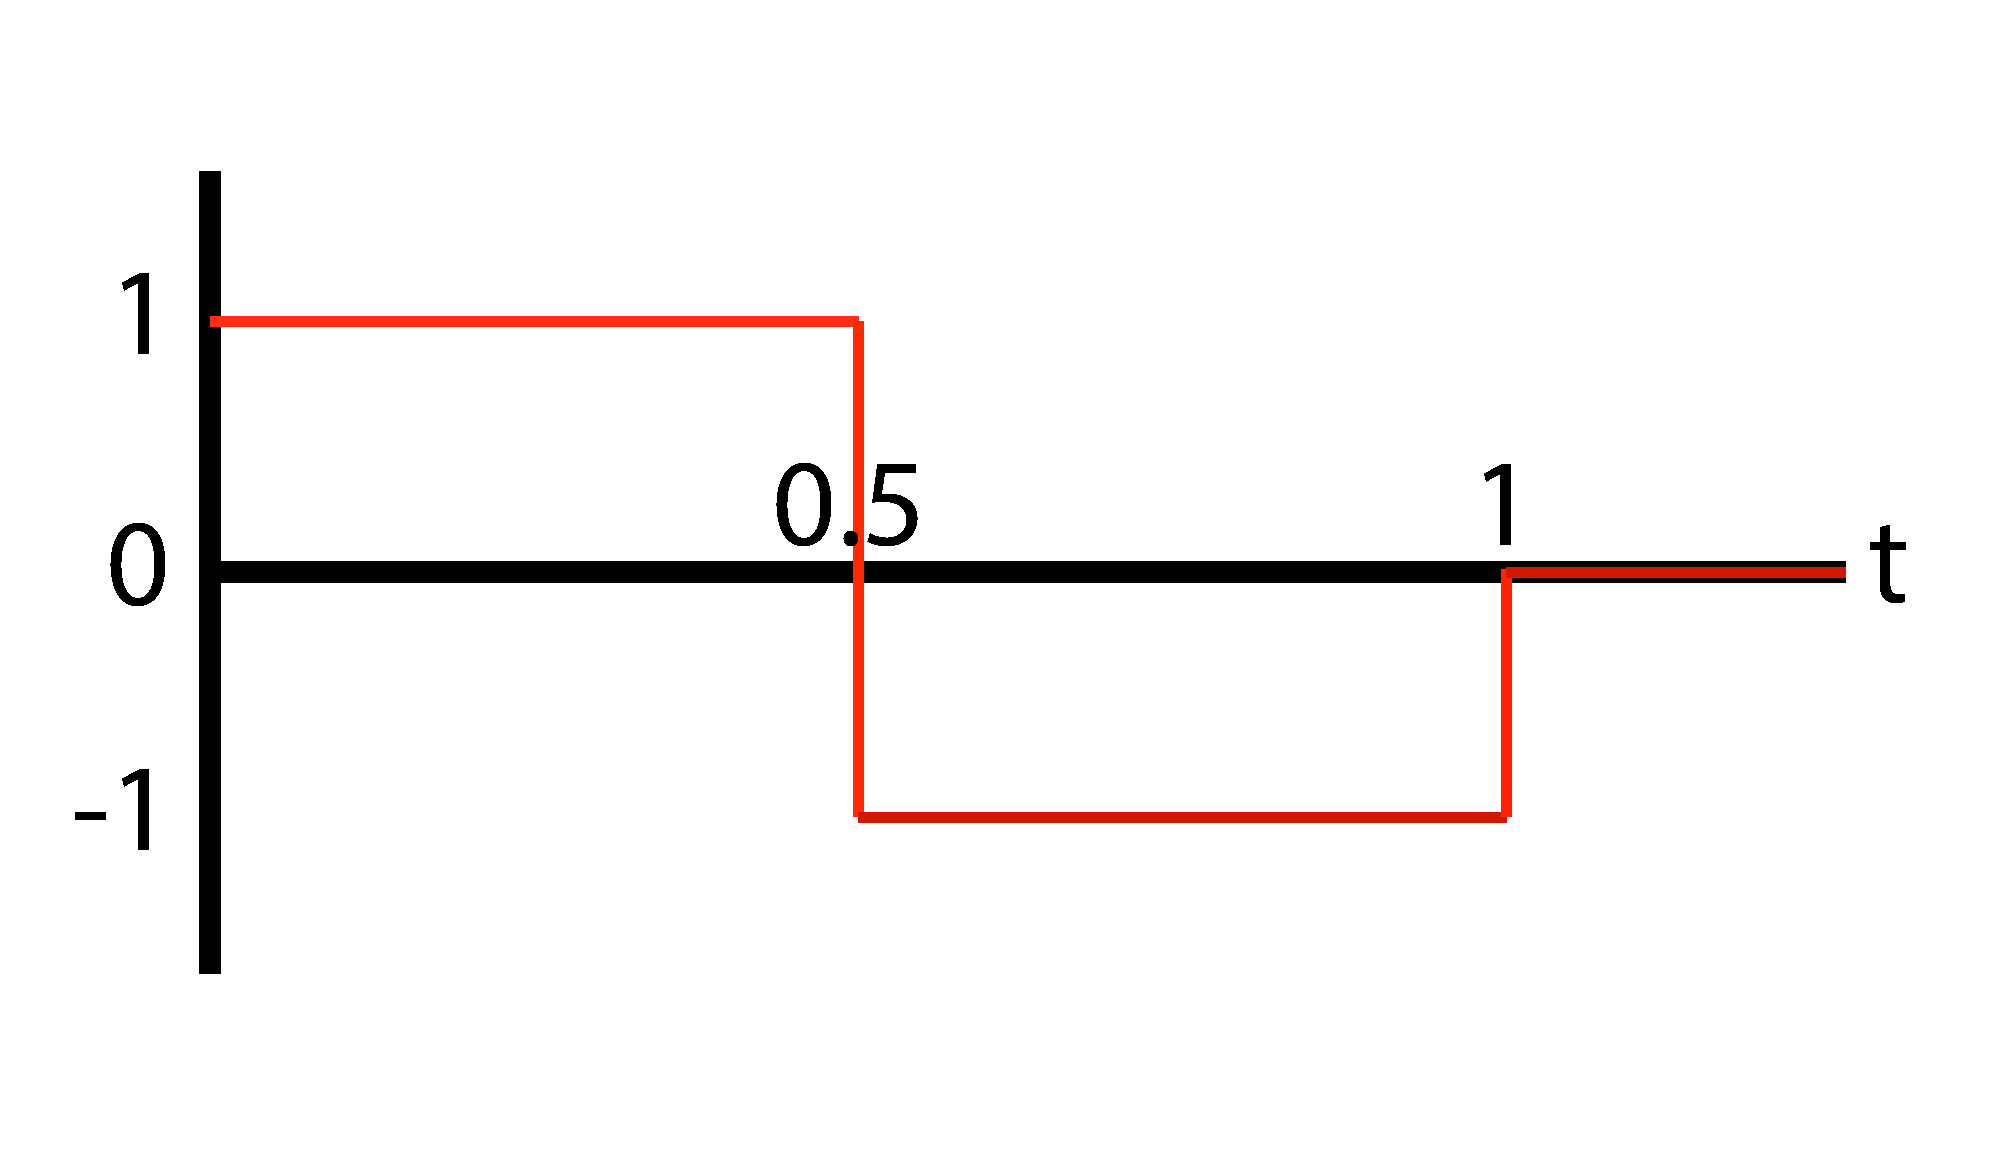
\includegraphics[height=3cm]{content/HaarWavelet.pdf}
	\end{minipage}	
	\begin{minipage}[c]{0.3\textwidth}
		\[
			\psi(t)=\begin{cases} 1 \quad 0 \leq t < \frac{1}{2}\\ -1 \quad \frac{1}{2} \leq t < 1  \end{cases}  
		\]
	\end{minipage}
\end{center}


\[  
	\psi_{m,n}(t)=\frac{1}{\sqrt{2^m}} \cdot \psi(\frac{t}{2^m} - n) = 2^{-m/2} \cdot \psi(2^{-m}t-n) 
	\qquad \qquad
	\psi_{m,n}  = \begin{cases} 
	\frac{1}{\sqrt{2^m}} \qquad 2^m n \leq t < 2^m(n+\frac{1}{2}) \\ 
	\frac{-1}{\sqrt{2^m}} \qquad 2^m(n+\frac{1}{2}) \leq t < 2^m(n+1)
	\end{cases}
\]

\[ 
	\nu_{m,n} = \langle \psi_{m,n} | f \rangle = \int_{-\infty}^{\infty}\psi_{m,n}(t) \cdot f(t) \,\mathrm{d}t
	\qquad \Longleftrightarrow \qquad
	f(t)=\sum_{m,n \in \mathbb{Z}} \nu_{m,n} \cdot \psi{m,n}
\]
	
\[  
	||f||^2 = \sum_{m,n \in \mathbb{Z}} |\nu_{m,n}|^2 \qquad \qquad ||f-f_N||^2 = ||f - \sum_{m,n \in \mathbb{Z}}^N \nu_{m,n} \cdot \psi_{m,n}||^2 = \sum_{k=N+1}^{\infty} |c_k|^2
\]

\textbf{Haar-Transformation:}
\begin{enumerate}
	\item Funktion abtasten bei $2^m(n+1/2)$ im Intervall $[a,b] \qquad u_{m,n}\approx \sqrt{2^m}f(2^m[n+1/2])$ 
	\item Die abgetastete Sequenz mit 0 auffüllen bis zu einer Zweierpotenz
	\item In jedem Schritt $u_{m+k+1}, \nu_{m+k+1}$ berechnen
\end{enumerate}

Schnelle Haar-Transformation:
\[  
	u_{m,n} = \dfrac{u_{m,2n}+u_{m,2n+1}}{\sqrt{2}} 
	\qquad \qquad
	\nu_{m,n} = \dfrac{u_{m,2n}-u_{m,2n+1}}{\sqrt{2}}
\]
